\documentclass[conference]{IEEEtran}
\IEEEoverridecommandlockouts

\usepackage{cite}
\usepackage{amsmath,amssymb,amsfonts}
\usepackage{graphicx}
\usepackage{booktabs}
\usepackage{array}
\usepackage{textcomp}
\usepackage{xcolor}
\usepackage{url}
\graphicspath{{figures/}}
% compact mean$\pm$std cell: \ms{mean}{std} -> mean with small subscript std
\newcommand{\ms}[2]{$#1_{\pm#2}$}

\begin{document}

\title{Gated Position-Aided Fusion for Blockage-Robust\\ Neural Beam Selection in 5G NR mmWave Systems}

\author{\IEEEauthorblockN{Furkan Yakkan and Akif Hasdemir}
\IEEEauthorblockA{Graduate School of Engineering and Science\\
Abdullah G\"ul University, Kayseri, T\"urkiye\\
Email: furkan.yakkan@agu.edu.tr; akif.hasdemir@agu.edu.tr}
\thanks{Both authors contributed equally to this work.}}

\maketitle

\begin{abstract}
Beam selection in millimeter-wave (mmWave) 5G New Radio (NR) requires sweeping a
large beam-pair codebook, incurring substantial initial-access overhead. A
well-known neural approach predicts the full reference-signal-received-power
(RSRP) profile over all beam pairs from a small set of downsampled RSRP
measurements, enabling a top-$K$ sweep over only the most promising beams. We
first reproduce this regression benchmark on the standardized TR~38.901 urban
macrocell scenario, attaining $90\%$ top-$K$ accuracy at $K=13$ ($81.4\%$
sweep-overhead reduction). We then investigate whether fusing the already
available user-equipment (UE) position with the sparse RSRP improves selection.
Contrary to the common multi-modal intuition, we find that on \emph{clean} RSRP
the single-modality predictor is already near-optimal: position fusion, learned
beam sampling, a beam-grid convolutional reconstruction, and uncertainty-aware
adaptive-$K$ all fail to beat it. The value of the position modality emerges only
when the RSRP modality is \emph{degraded}. Building on this, we propose a
\emph{gated residual position-aided fusion} network in which a position-driven
correction is added to the RSRP-based estimate through a learned gate. The gate
preserves clean-data accuracy at no cost while the residual path delivers a
consistent $2$--$4$ percentage-point top-$K$ accuracy gain under mmWave beam
blockage (when $6$--$12$ of the $14$ measured beams are lost). An architecture
ablation confirms the gate is responsible for the no-regret behavior. The result
is a practical, no-regret robustness improvement for blockage-prone mmWave links.
\end{abstract}

\begin{IEEEkeywords}
5G NR, millimeter wave, beam management, beam selection, deep learning,
multi-modal fusion, beam blockage, RSRP.
\end{IEEEkeywords}

\section{Introduction}
Millimeter-wave (mmWave) bands are central to 5G NR and 6G for their large
bandwidths, but their high pathloss and susceptibility to blockage demand highly
directional beamforming~\cite{xue2024survey}. During initial access, the
gNB and UE must establish a good transmit/receive beam pair, classically through
an exhaustive synchronization-signal-block (SSB) beam sweep over the full
codebook. With many narrow beams, this sweep dominates initial-access latency and
overhead, motivating machine-learning methods that predict good beams from
partial or out-of-band observations~\cite{heng2019mlbeam,klautau2018itadata}.

Two broad families have emerged. \emph{In-band} methods exploit RSRP or channel
measurements~\cite{sim2020sub6,polese2021deepbeam}; they are accurate when
measurements are reliable. \emph{Side-information} methods exploit position,
LiDAR, radar, vision, or sub-6\,GHz channels~\cite{klautau2019lidar,
rezaie2022location,alkhateeb2023deepsense,demirhan2022radar,deng2025scanbest};
they are robust to RF impairments but typically achieve lower peak accuracy.
A widely used in-band formulation, distributed as a reference example by
MathWorks,\footnote{This is the project's designated benchmark (Option~B,
\emph{Neural Network for Beam Selection}).} casts beam selection as RSRP-profile
\emph{regression}: a neural network maps a downsampled subset of RSRP
measurements to the full per-beam-pair RSRP profile, after which only the top-$K$
predicted beams are swept. This example was \emph{recently updated} from an
earlier position-input classifier to the regression formulation we reproduce; we
reconcile the two versions in Section~\ref{sec:benchmark}.

In this work we take this regression benchmark as our starting point and ask a
simple question: \emph{does adding the UE position---already available at the
network---improve beam selection?} Our investigation yields a nuanced and, we
believe, instructive answer. The contributions are:
\begin{itemize}
\item We reproduce the SSB-RSRP regression benchmark on the TR~38.901 urban
macrocell (UMa) scenario and confirm its headline operating point: $90\%$
top-$K$ accuracy at $K=13$, i.e. an $81.4\%$ reduction in beam-sweep overhead,
with average RSRP within $0.24$\,dB of exhaustive search
(Section~\ref{sec:benchmark}).
\item We show that, on clean RSRP, the single-modality predictor is at the
achievable ceiling: naive position fusion, statistically ``optimized'' beam
sampling, a 2D beam-grid convolutional reconstruction, and uncertainty-aware
adaptive-$K$ all fail to improve it (Section~\ref{sec:negative}). This isolates
\emph{where} a second modality can help.
\item We propose a \emph{gated residual position-aided fusion} network and an
impairment-aware training procedure (Section~\ref{sec:method}). It is a
\emph{no-regret} design: it matches the RSRP-only model on clean data and
improves top-$K$ accuracy by $2$--$4$ points under beam blockage. An architecture
ablation shows the gate is what preserves the clean-data parity
(Section~\ref{sec:results}). As a finding, the learned gate converges to a
near-constant scale: in this single-impairment setting a fixed-scale residual
position path is sufficient and no-regret, and genuinely adaptive gating would be
expected only when position reliability \emph{itself} varies---a direction we
outline in Section~\ref{sec:conclusion}.
\end{itemize}

The complete MATLAB implementation, trained models, and the \LaTeX{} source of
this paper are publicly available.\footnote{\url{https://github.com/fyakkan/neural-beam-selection}}

\section{Related Work (Literature Review)}\label{sec:related}
Early ML beam-selection work posed the task as classification of the best beam
(pair) from side information such as UE position or LiDAR
\cite{heng2019mlbeam,klautau2018itadata,klautau2019lidar}, a classification line
that continues on real V2I data~\cite{biliaminu2024v2i}. Position/location-aided
prediction was extended to 3D beam selection with orientation
information~\cite{rezaie2022location}, and to real-world GPS-based prediction on
the DeepSense~6G testbed~\cite{alkhateeb2023deepsense}. Out-of-band approaches
predict mmWave beams (and blockages) from sub-6\,GHz channels
\cite{sim2020sub6,alrabeiah2020sub6blockage,deng2025scanbest}, reporting large
overhead reductions (e.g.\ $\sim$79\% in~\cite{sim2020sub6}). Sensing-aided
prediction using radar~\cite{demirhan2022radar} and LiDAR~\cite{jiang2023lidar}
has been demonstrated on real V2I data, and waveform-learning approaches such as
DeepBeam~\cite{polese2021deepbeam} reduce beam-management latency without
coordination, while entropy-based probing-beam selection cuts measurement
overhead~\cite{meng2024entropy}. A parallel line predicts \emph{blockage} for proactive handoff
\cite{alkhateeb2018blockage,wu2022blockage}, and recent work exploits temporal
correlation for vehicular beam management~\cite{oliveira2025temporal}. Surveys
\cite{xue2024survey} and the 3GPP study on AI/ML for the NR air
interface~\cite{tr38843} provide broader context.

Table~\ref{tab:related} summarizes representative methods by input modality and
reported benefit. Two gaps motivate our work. First, multi-modal fusion is
typically studied with rich external sensors (camera/LiDAR/radar) on vehicular
data, not with the \emph{already-available} UE position fused into the canonical
SSB-RSRP regression. Second, prior fusion work emphasizes peak accuracy on
nominal data rather than \emph{robustness as a function of measurement
reliability}. We address both, and---importantly---report the negative result
that on clean RSRP the position modality is redundant, which clarifies that the
fusion payoff is a robustness, not an accuracy, story.

\begin{table*}[t]
\centering
\caption{Representative ML beam-management methods (2018--2025).}
\label{tab:related}
\begin{tabular}{@{}p{3.0cm}p{2.4cm}p{4.0cm}p{4.6cm}@{}}
\toprule
\textbf{Work (year)} & \textbf{Modality} & \textbf{Approach} & \textbf{Reported benefit} \\
\midrule
Heng \& Andrews~\cite{heng2019mlbeam} (2019) & Position & NN beam alignment & ML-assisted alignment vs.\ exhaustive sweep \\
Klautau \emph{et al.}~\cite{klautau2019lidar} (2019) & LiDAR & DL beam selection & Out-of-band beam selection \\
Sim \emph{et al.}~\cite{sim2020sub6} (2020) & Sub-6\,GHz & DL beam selection (NR/6G) & $\sim$79\% sweep-overhead reduction \\
Alrabeiah \& Alkhateeb~\cite{alrabeiah2020sub6blockage} (2020) & Sub-6\,GHz & DL beam + blockage prediction & $>$90\% blockage prediction \\
Rezaie \emph{et al.}~\cite{rezaie2022location} (2022) & Position + orientation & DL 3D beam set selection & Location/orientation-aided selection \\
Polese \emph{et al.}~\cite{polese2021deepbeam} (2021) & Waveform/RF & Coordination-free beam mgmt & $\sim$7$\times$ lower latency (default config) \\
Demirhan \& Alkhateeb~\cite{demirhan2022radar} (2022) & Radar & DL beam prediction & Real-world radar-aided prediction \\
Jiang \emph{et al.}~\cite{jiang2023lidar} (2023) & LiDAR & DL future-beam prediction & $\sim$90\% overhead reduction (V2I) \\
Wu \emph{et al.}~\cite{wu2022blockage} (2022) & In-band power & Moving-blockage prediction & $>$85\% blockage accuracy \\
Oliveira \emph{et al.}~\cite{oliveira2025temporal} (2025) & Position + time & RNN temporal beam mgmt & Up to 50\% overhead reduction \\
Biliaminu \emph{et al.}~\cite{biliaminu2024v2i} (2024) & Position/geo & ML multiclass beam classification & Beam prediction on real V2I (DeepSense) \\
Meng \emph{et al.}~\cite{meng2024entropy} (2024) & RSRP/probing & Entropy-based probing + DL prediction & Reduced probing/measurement overhead \\
\textbf{This work} & \textbf{Sparse RSRP + position} & \textbf{Gated residual fusion} & \textbf{No clean-data cost; $+2$--$4$ pts under blockage} \\
\bottomrule
\end{tabular}
\end{table*}

\section{System Model and Regression Benchmark}\label{sec:benchmark}

\subsection{Scenario and beam codebook}
We adopt the TR~38.901 UMa scenario~\cite{tr38901} in frequency range~2 (FR2) at
a carrier of $30$\,GHz, following the AI/ML system-level assumptions of
TR~38.843~\cite{tr38843}. The gNB uses
a $4\times8$ cross-polarized panel and the UE a $1\times4$ panel, yielding
$N_{\mathrm{tx}}=10$ transmit beams and $N_{\mathrm{rx}}=7$ receive beams, for a
total of $N_b=N_{\mathrm{tx}}N_{\mathrm{rx}}=70$ beam pairs covering a
$120^\circ$ sector. For each UE location, SSB-based beam sweeping yields an RSRP
value for every beam pair, forming an RSRP matrix
$\mathbf{R}\in\mathbb{R}^{7\times 10}$; we index beam pairs by the column-major
linear index $b\in\{1,\dots,70\}$ of $\mathbf{R}$. We use the official
pre-recorded dataset of $15{,}000$ training and $500$ test UE locations. Blocked
beams appear as $-\infty$ RSRP ($4.6\%$ of entries; $\sim$10\% of locations have
at least one blocked beam among the sampled set); we floor them to $-120$\,dB for
network inputs/targets.

\subsection{Regression formulation}
Let $\mathbf{r}\in\mathbb{R}^{70}$ be the vectorized RSRP profile of a UE.
A fixed downsampling selects every fifth beam pair, giving
$\mathcal{S}=\{1,6,11,\dots,66\}$ with $|\mathcal{S}|=14$ measured beams and input
$\mathbf{x}=\mathbf{r}_{\mathcal{S}}\in\mathbb{R}^{14}$. A network
$f_\theta:\mathbb{R}^{14}\!\to\!\mathbb{R}^{70}$ regresses the full profile
$\hat{\mathbf{r}}=f_\theta(\mathbf{x})$; targets are min-max normalized to
$[-1,1]$ and the output layer is $\tanh$. At inference, the $K$ beams with the
largest predicted RSRP are swept and the one with the strongest \emph{actual}
RSRP is selected. The metrics are the top-$K$ accuracy (the fraction of UEs whose
true-optimal beam is among the $K$ predicted) and the average selected RSRP.

The benchmark network is a four-hidden-layer multilayer perceptron (MLP) of width
$96$ with leaky-ReLU activations and $z$-score input normalization, trained with
Adam to minimize mean-squared error. Position is \emph{not} an input to the
network; it is used only by a $K$-nearest-neighbor (KNN) benchmark, alongside
Statistical and Random baselines.

\subsection{Reproduction results}
Table~\ref{tab:benchmark} reports the reproduced metrics and Fig.~\ref{fig:base}
the top-$K$ accuracy curves. The neural predictor reaches $90.0\%$ top-$K$
accuracy at $K=13$---sweeping fewer than one quarter of the $70$ beam pairs, an
$81.4\%$ overhead reduction---and $97.4\%$ at $K=30$. Its average RSRP at $K=13$
is $-23.21$\,dB, within $0.24$\,dB of the exhaustive optimum ($-22.97$\,dB) and
well above KNN ($-25.29$\,dB). The neural method dominates KNN, Statistical, and
Random across all $K$, reproducing the published behavior and validating our
pipeline.

\emph{Reconciliation with the original formulation.} The MathWorks example was
originally a position-input multi-class \emph{classifier}---predicting the optimal
beam-pair index directly from the UE's 3D coordinates---but has since been updated
to the RSRP-profile \emph{regression} formulation reproduced above. We adopt the
current (regression) version for two reasons: it is the live reference, and it
cleanly separates the in-band (RSRP) and side-information (position) modalities,
which is exactly what our fusion study requires (position becomes an \emph{added}
modality rather than the sole input). We also re-implement rather than re-run the
shipped code: the online example uses a wider $64$--$128$--$256$--$128$ ReLU
network with global-max input normalization on a $20{,}000/700$ split, whereas we
use a compact width-$96$ leaky-ReLU $z$-score MLP on the $15{,}000/500$
pre-recorded dataset bundled with the example. Despite these differences, our
re-implementation reproduces the published operating point ($90\%$ top-$K$
accuracy at $K=13$), confirming functional equivalence; the RSRP-only reference
used throughout our experiments shares this width-$96$ architecture, so all
comparisons are internally fair.

\begin{table}[t]
\centering
\caption{Reproduced benchmark metrics (15k/500, $K=13$ unless noted).}
\label{tab:benchmark}
\begin{tabular}{@{}lccc@{}}
\toprule
Metric & Neural & KNN & Optimal \\
\midrule
Top-$K$ reaches 90\% at & $K=13$ & -- & -- \\
Overhead reduction @\,$K{=}13$ & 81.4\% & -- & -- \\
Top-$K$ accuracy @\,$K{=}13$ & \textbf{90.0\%} & 37.8\% & -- \\
Top-$K$ accuracy @\,$K{=}30$ & 97.4\% & -- & -- \\
Avg.\ RSRP @\,$K{=}13$ (dB) & \textbf{$-23.21$} & $-25.29$ & $-22.97$ \\
\bottomrule
\end{tabular}
\end{table}

\begin{figure}[t]
\centering
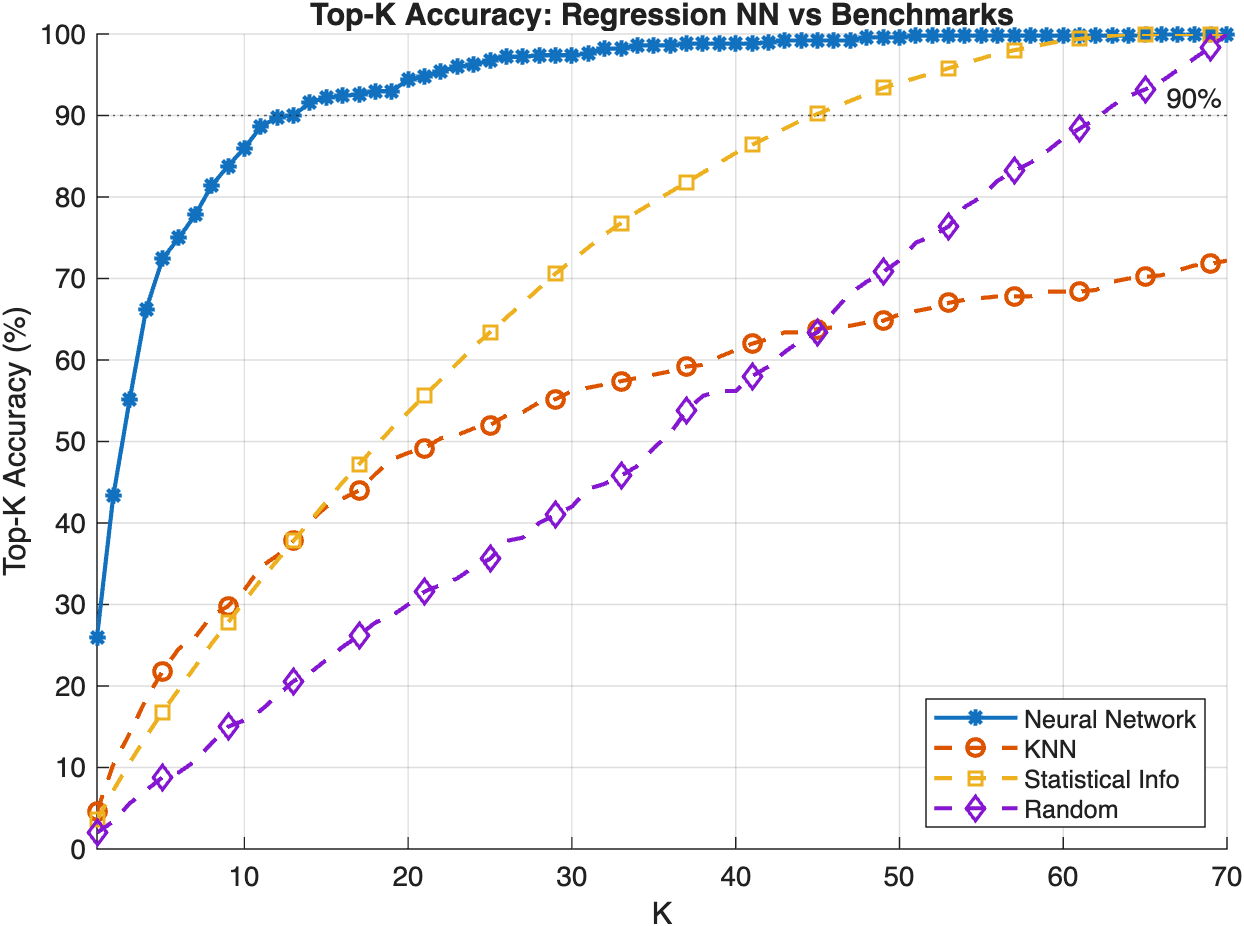
\includegraphics[width=0.9\columnwidth]{baseline_topk_accuracy.png}
\caption{Reproduced benchmark: top-$K$ accuracy of the RSRP-regression network
vs.\ KNN, Statistical, and Random baselines. The network reaches $90\%$ at
$K=13$.}
\label{fig:base}
\end{figure}

\section{Where a Second Modality Does (Not) Help}\label{sec:negative}
Before designing a fusion model, we tested whether the benchmark can be improved
on \emph{clean} RSRP along four axes, each under identical data, splits, and
seeds:
\begin{enumerate}
\item \textbf{Naive position fusion}: a two-branch network ingesting the $14$
RSRP values and the 3D UE position. Result: a tie within noise on clean data
($+0.8$ at $K{=}13$, $-3.0$ at $K{=}5$).
\item \textbf{Learned/statistical beam sampling}: replacing the uniform
every-fifth sampling with the $14$ highest-variance, most-frequently-optimal, or
strongest-mean beams. All were \emph{worse} (e.g.\ $K_{90}{=}39$ vs.\ $13$),
because clustered beams lose spatial coverage; uniform sampling is near-optimal.
\item \textbf{2D beam-grid CNN}: treating sparse sensing as inpainting on the
$7\times10$ (Rx$\times$Tx) RSRP image with observed-value and mask channels.
Result: worse at the operating point ($K_{90}{=}16$ vs.\ $13$).
\item \textbf{Uncertainty-aware adaptive-$K$}: a nucleus rule over the predicted
profile to choose a per-UE $K$. Result: negligible ($\leq{+}0.6$ pts at matched
mean overhead).
\end{enumerate}
The common explanation is that the optimal beam is determined by the channel,
which the RSRP directly measures; the UE position predicts the optimal beam only
weakly (KNN attains $37.8\%$ at $K{=}13$). Hence, when RSRP is clean, position is
largely \emph{redundant}, and richer architectures merely add variance. This
motivates targeting the regime where RSRP is unreliable.

\section{Proposed Method: Gated Residual Position-Aided Fusion}\label{sec:method}

\subsection{Beam-blockage model}
Practical mmWave sweeps lose measurements to blockage and missed detections. We
model this by, for each UE, setting $n_B$ of the $14$ measured beams (chosen
uniformly at random) to the floor value, plus a small Gaussian RSRP measurement
noise. The number of blocked input beams $n_B$ parameterizes the impairment
severity; $n_B$ large corresponds to only a handful of reliably measured beams.
We note that this model drops beams independently and uniformly at random,
whereas physical mmWave blockage is spatially \emph{correlated}---a single
obstruction tends to occlude a contiguous set of beam directions. We adopt the
i.i.d.\ model as our primary setting and separately verify robustness under
correlated (contiguous) blockage in Section~\ref{sec:corr}.

\subsection{Architecture}
The proposed network has two encoders. An RSRP encoder maps $\mathbf{x}$ to a
primary estimate $\mathbf{b}=g_{\text{base}}(\mathbf{x})\in\mathbb{R}^{70}$
(structurally the RSRP-only path). A position encoder maps the 3D UE position
$\mathbf{p}$ to a correction $\mathbf{c}=g_{\text{corr}}(\mathbf{p})\in
\mathbb{R}^{70}$. A gate $\mathbf{g}=\sigma(g_{\text{gate}}([\mathbf{h}_r,
\mathbf{h}_p]))\in(0,1)^{70}$, computed from both encoder features
$\mathbf{h}_r,\mathbf{h}_p$, weights the correction. The output is
\begin{equation}
\hat{\mathbf{r}} \;=\; \tanh\!\big(\mathbf{b} \;+\; \mathbf{g}\odot\mathbf{c}\big),
\label{eq:gated}
\end{equation}
where $\odot$ is the elementwise product. The residual-plus-gate structure lets
the network recover the strong RSRP-only estimate (by suppressing
$\mathbf{g}\odot\mathbf{c}$) when RSRP is reliable, and inject the position prior
when it is not. The RSRP encoder uses two width-$96$ layers, the position encoder
two width-$32$ layers, and the gate a width-$64$ layer; all use leaky-ReLU.

\subsection{Impairment-aware training}
Both the proposed model and the RSRP-only reference are trained with the
\emph{same} blockage augmentation: per sample, $n_B\sim\mathcal{U}\{0,\dots,8\}$
beams are dropped and light noise is added. This teaches the models to operate
across blockage levels and makes the comparison differ only in the position
modality. Networks are trained with Adam ($300$ epochs, mini-batch $512$, initial
learning rate $10^{-3}$ with piecewise decay).

\section{Experimental Results}\label{sec:results}

\subsection{Experimental setup}
All experiments use the TR~38.901 UMa scenario at $30$\,GHz (FR2), with a
$4\times8$ gNB panel and $1\times4$ UE panel giving $70$ beam pairs; the network
input is the $14$ uniformly downsampled RSRP measurements. We use the official
pre-recorded dataset of $15{,}000$ training and $500$ test UE locations, holding
out $10\%$ of training data for validation ($13{,}500/1{,}500/500$
train/validation/test). All networks are trained with Adam for $300$ epochs,
mini-batch $512$, initial learning rate $10^{-3}$ with piecewise decay
($\times0.5$ every $80$ epochs), minimizing mean-squared error on the
$[-1,1]$-normalized RSRP profile; the proposed and RSRP-only models additionally
use blockage augmentation ($n_B\sim\mathcal{U}\{0,\dots,8\}$). Blockage-robustness
results are averaged over $10$ independent random blockage draws (we report the
mean and standard deviation). Experiments run in MATLAB R2025b (Deep Learning, 5G,
Communications, Phased Array System, Statistics and Machine Learning, DSP System,
and Signal Processing Toolboxes); the networks are compact enough to train on CPU
in a few minutes each (no GPU required).

\subsection{Robustness to beam blockage}
Fig.~\ref{fig:blockacc} and Table~\ref{tab:blockage} report top-$K$ accuracy
($K=13$, averaged over $10$ random blockage draws) versus the number of blocked
input beams. On clean inputs ($n_B=0$) the proposed fusion matches the RSRP-only
model ($89.4\%$ vs.\ $89.2\%$): the position modality incurs \emph{no}
cost.\footnote{The RSRP-only clean accuracy here ($89.2\%$) is marginally below
the $90.0\%$ of Section~\ref{sec:benchmark} because the models in this section are
trained with blockage augmentation, which costs $\sim$0.8 points on clean inputs;
the width sweep in Section~\ref{sec:results} likewise reports $89.6\%$ for the
narrowest (width-$32$) network.} As
beams are blocked, the fusion pulls ahead, with a consistent $+2$ to $+3.8$-point
advantage for $n_B\in[6,12]$ (e.g.\ $39.7\%$ vs.\ $35.9\%$ at $n_B=10$). The
position-only KNN is blockage-immune but flat at $37.8\%$, far below both
networks except under extreme blockage. Fig.~\ref{fig:blocktopk} shows that, at a
representative $n_B=8$, the fusion dominates the RSRP-only model across the entire
$K$ range. Quantifying significance across the $10$ draws (Table~\ref{tab:blockage}):
the small differences at $n_B\le 4$ ($+0.2$, $-1.1$, $+0.6$) lie within one
standard deviation and are not statistically meaningful, whereas the gains for
$n_B\ge 5$ ($+2.0$ to $+3.8$ over $n_B\in[6,12]$) consistently exceed the
per-draw standard deviation and constitute the real effect. (The $\pm0.0$ std at
$n_B{=}0$ is exact: with no beams blocked the clean input is identical across
draws.) Note that the models are trained with $n_B\sim\mathcal{U}\{0,\dots,8\}$,
so the results at $n_B\in\{10,12\}$ additionally probe generalization \emph{beyond}
the trained blockage range, where the fusion advantage is largest.

\begin{table*}[t]
\centering
\caption{Top-$K$ accuracy ($K{=}13$, \%, mean$\pm$std over 10 blockage draws) vs.\ number of blocked input beams.}
\label{tab:blockage}
\footnotesize
\begin{tabular}{@{}lccccccc@{}}
\toprule
\# blocked & 0 & 2 & 4 & 6 & 8 & 10 & 12 \\
\midrule
RSRP-only & \ms{89.2}{0.0} & \ms{84.6}{1.1} & \ms{78.1}{2.2} & \ms{69.8}{1.5} & \ms{56.0}{1.6} & \ms{35.9}{2.4} & \ms{22.3}{0.9} \\
Gated fusion & \ms{89.4}{0.0} & \ms{83.5}{1.0} & \ms{78.7}{1.1} & \ms{72.1}{1.7} & \ms{57.9}{2.0} & \ms{39.7}{1.7} & \ms{24.9}{1.4} \\
Gain (pts) & $+0.2$ & $-1.1$ & $+0.6$ & $+2.3$ & $+2.0$ & $+3.8$ & $+2.6$ \\
\bottomrule
\end{tabular}
\end{table*}

\begin{figure}[t]
\centering
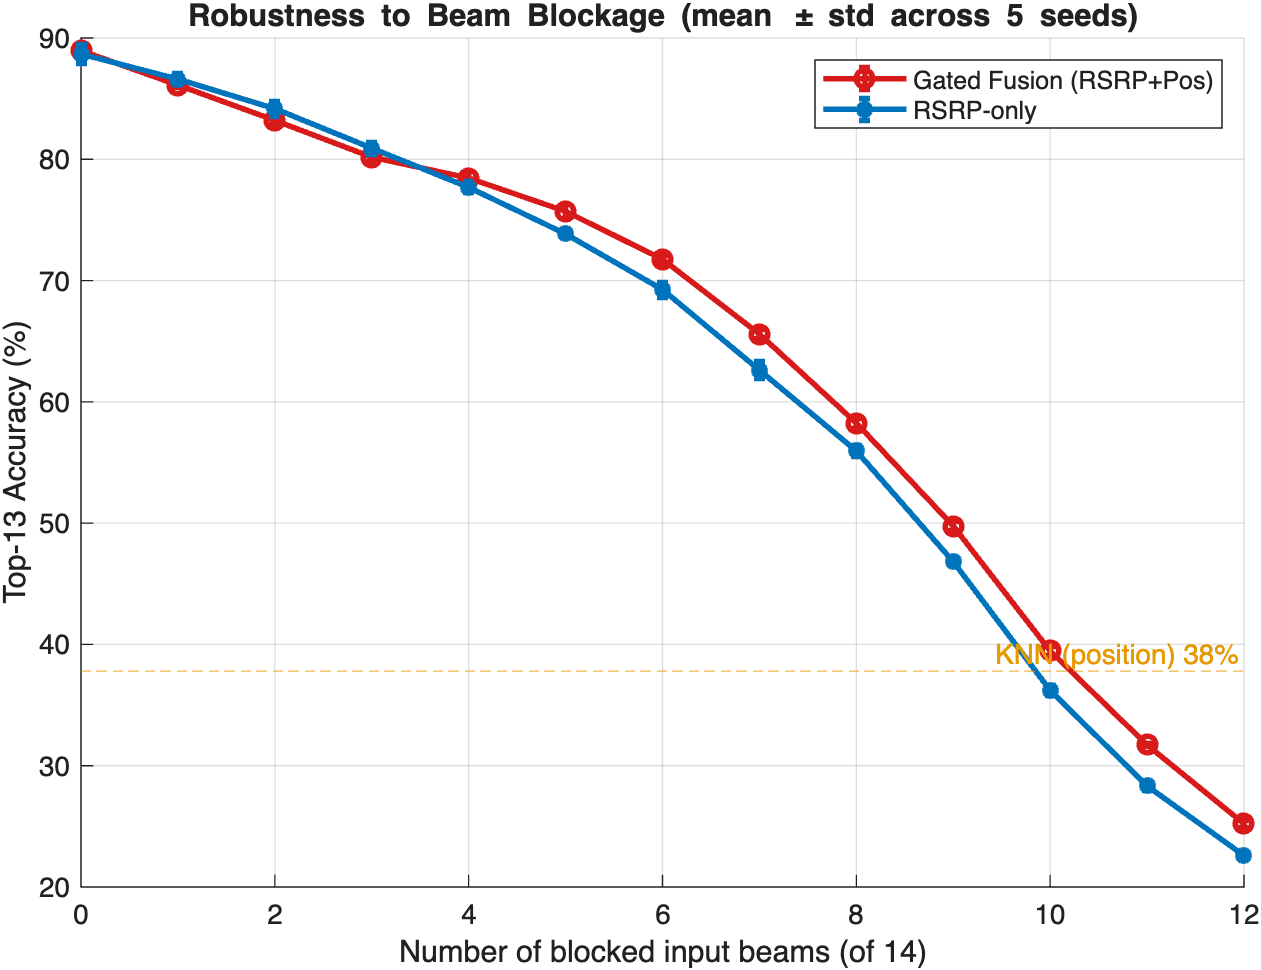
\includegraphics[width=0.9\columnwidth]{novel_blockage_accuracy.png}
\caption{Top-$K$ accuracy ($K{=}13$) vs.\ number of blocked input beams; error
bars are $\pm1$ standard deviation over $10$ blockage draws. The gated fusion
matches RSRP-only when clean and improves it under blockage; KNN (position only)
is flat.}
\label{fig:blockacc}
\end{figure}

\begin{figure}[t]
\centering
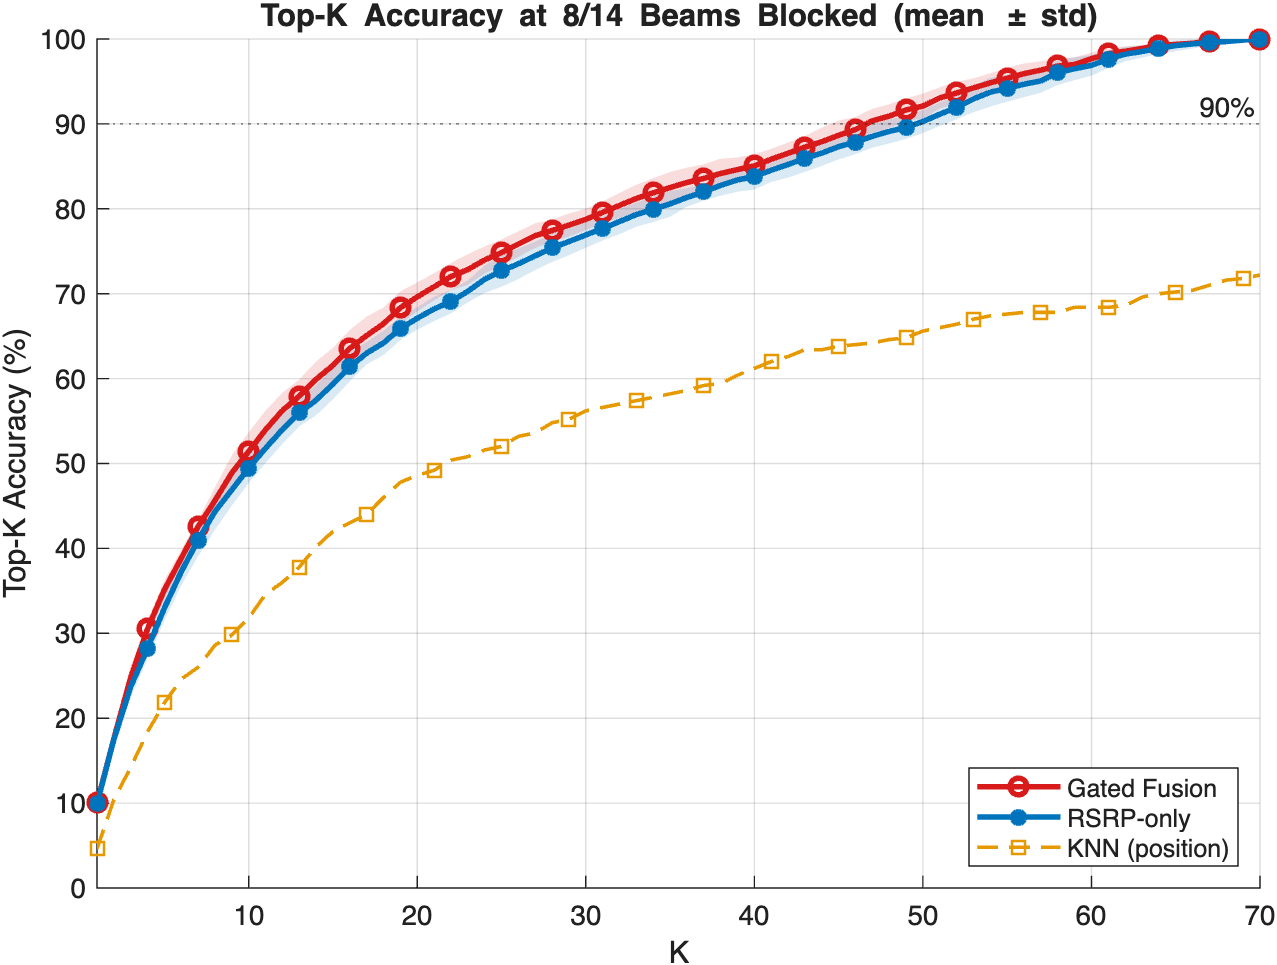
\includegraphics[width=0.9\columnwidth]{novel_blockage_topk.png}
\caption{Top-$K$ accuracy vs.\ $K$ at a representative $8/14$ blocked input beams;
shaded bands are $\pm1$ standard deviation over $10$ draws. The gated fusion
dominates the RSRP-only model across $K$; both far exceed position-only KNN.}
\label{fig:blocktopk}
\end{figure}

\subsection{Architecture ablation: is the gate needed?}
Table~\ref{tab:ablarch} compares four fusion variants trained identically:
RSRP-only, concatenation fusion, plain residual ($\mathbf{g}\!=\!1$ in
\eqref{eq:gated}), and the proposed gated residual. The plain residual already
provides most of the blockage robustness but costs $1.2$ points on clean data
($88.0\%$ vs.\ $89.2\%$). The gate restores clean parity ($89.4\%$) at equal
blockage robustness---this is precisely the role of the gate. Interestingly,
ungated \emph{concatenation} achieves the largest heavy-blockage gains
($45.9\%$ vs.\ $35.9\%$ at $n_B=10$) but sacrifices $4.8$ points on clean data,
i.e.\ it is \emph{not} no-regret. The gated residual occupies the best
clean-vs-robustness trade-off. Notably, the learned gate converges to a nearly
constant value ($\approx0.78$; Fig.~\ref{fig:gate}): rather than ``opening''
adaptively with blockage, it learns a fixed down-weighting of the position
correction that preserves clean accuracy while retaining robustness. We therefore
frame the gate's role as learning the (near-constant) optimal position-mixing
scale rather than performing per-sample adaptation: the contribution is a
no-regret residual fusion, and we expect genuinely adaptive gating to matter only
when position reliability \emph{itself} varies across users (e.g.\ GPS outages),
which we leave to future work (Section~\ref{sec:conclusion}).

\begin{table}[t]
\centering
\caption{Architecture ablation: top-$K$ accuracy ($K{=}13$, \%, mean$\pm$std over 10 draws) vs.\ blockage.}
\label{tab:ablarch}
\setlength{\tabcolsep}{4pt}
\footnotesize
\begin{tabular}{@{}lccccc@{}}
\toprule
\# blocked & 0 & 6 & 8 & 10 & 12 \\
\midrule
RSRP-only            & \ms{89.2}{0.0} & \ms{69.8}{1.5} & \ms{56.0}{1.6} & \ms{35.9}{2.4} & \ms{22.3}{0.9} \\
Concatenation        & \ms{84.4}{0.0} & \ms{69.7}{1.7} & \ms{59.8}{1.5} & \textbf{\ms{45.9}{1.2}} & \ms{29.1}{1.2} \\
Plain residual       & \ms{88.0}{0.0} & \ms{71.7}{1.8} & \ms{58.0}{2.1} & \ms{39.7}{1.8} & \ms{25.0}{1.4} \\
\textbf{Gated residual} & \textbf{\ms{89.4}{0.0}} & \ms{72.1}{1.7} & \ms{57.9}{2.0} & \ms{39.7}{1.7} & \ms{24.9}{1.4} \\
\bottomrule
\end{tabular}
\end{table}

\begin{figure}[t]
\centering
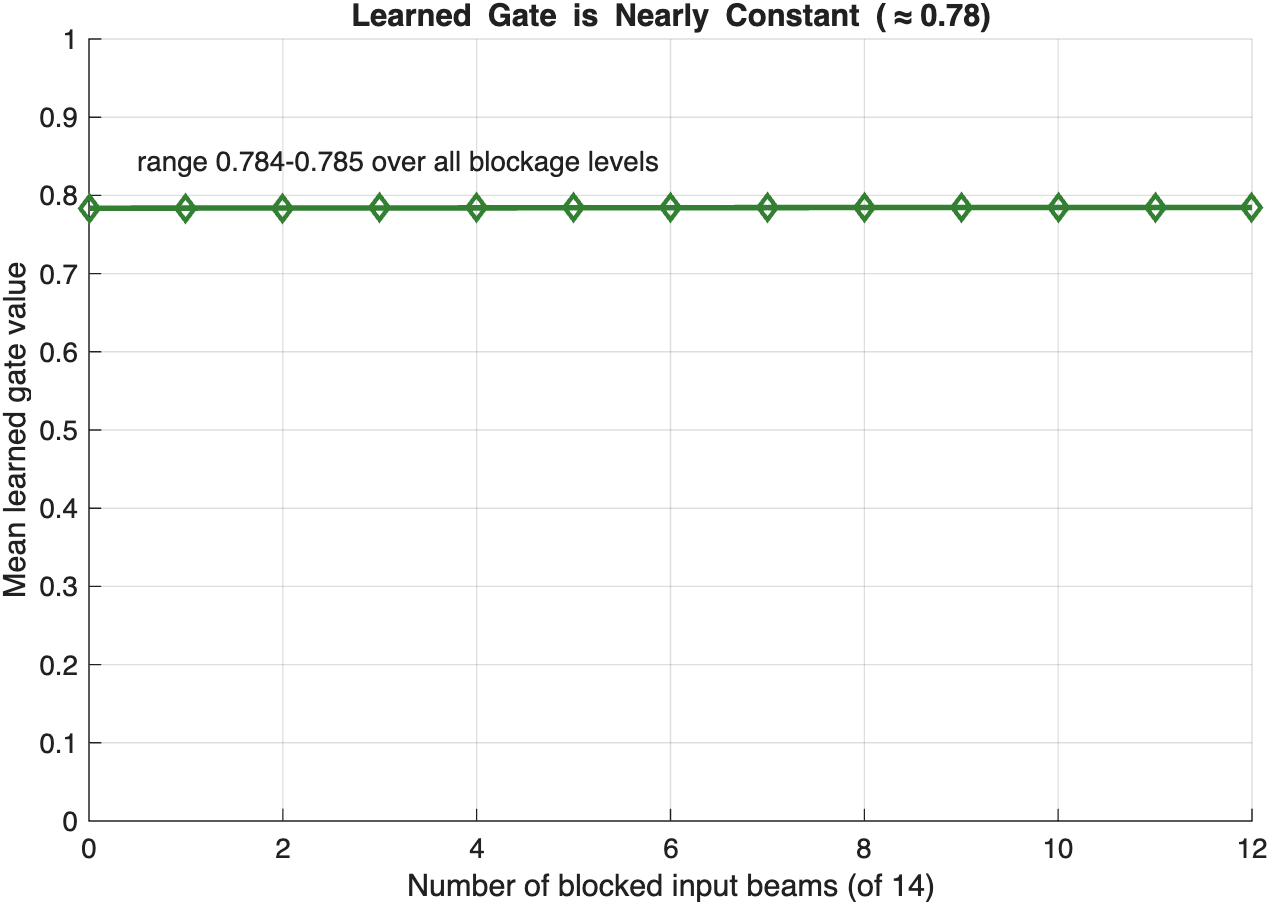
\includegraphics[width=0.9\columnwidth]{novel_gate_behavior.png}
\caption{The learned gate is nearly constant ($\approx0.78$) across blockage
levels: robustness arises from the always-on residual position path, not from
adaptive gating.}
\label{fig:gate}
\end{figure}

\subsection{Benchmark sensitivity (further analyses)}
We characterize the RSRP-only benchmark on clean data. \emph{Width}: increasing
the hidden width from $32$ to $384$ raises top-$K$ accuracy modestly ($89.6\%$ to
$91.8\%$ at $K{=}13$); width $96$ is a good accuracy/size balance. \emph{Depth}:
$2$--$4$ hidden layers perform equally ($\approx90\%$), while $6$--$8$ layers
degrade slightly (mild overfitting), justifying the four-layer choice.
\emph{UE density}: accuracy saturates by $\sim$$25\%$ of the training set
($3{,}375$ UEs, $90.6\%$), so the full $15$k set is comfortably in the saturated
regime---confirming that the clean-data ceiling is not a data-limited artifact.

\subsection{Robustness to correlated (contiguous) blockage}\label{sec:corr}
To probe a more realistic impairment, we additionally evaluate \emph{correlated}
blockage: rather than dropping the $n_B$ lost beams i.i.d., we drop a
\emph{contiguous} block of $n_B$ sampled beams (a single obstruction occluding a
contiguous angular region), reusing the same i.i.d.-trained models---i.e.\ a
test-time distribution shift. Fig.~\ref{fig:corr} shows that the gated-fusion
advantage not only persists but \emph{grows}: the gain rises to $+6.5$, $+7.3$,
and $+7.0$ points at $n_B=6,8,10$ (vs.\ $+2.3$, $+2.0$, $+3.8$ under i.i.d.\
blockage), well beyond the $\le\!2$-point per-draw standard deviation.
Intuitively, a contiguous gap removes an entire local region of the RSRP profile
that cannot be interpolated from neighboring samples, so the global position
prior contributes more. The method is thus, if anything, \emph{more} valuable
under the structured blockage expected in practice.

\begin{figure}[t]
\centering
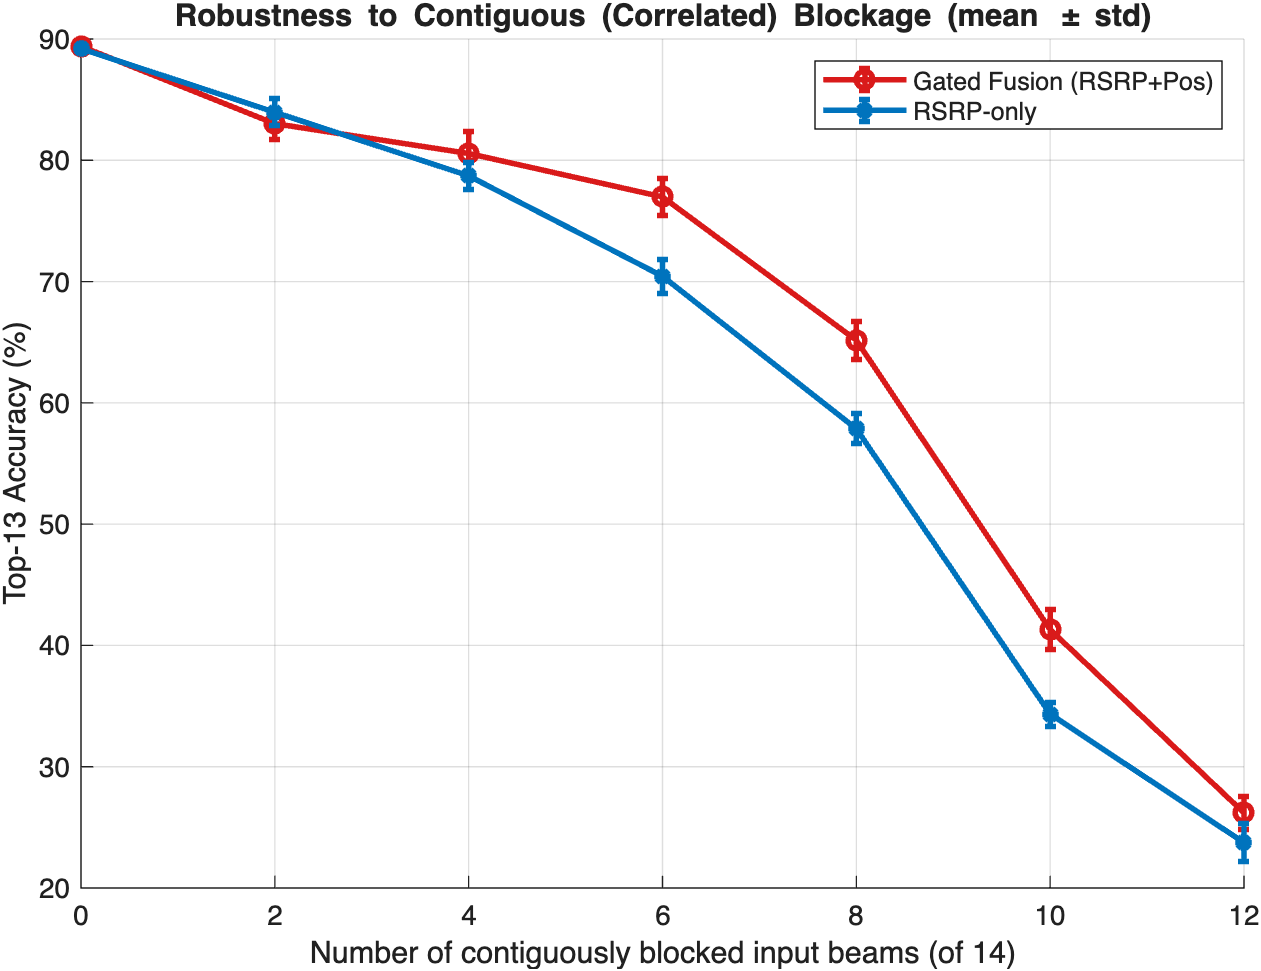
\includegraphics[width=0.9\columnwidth]{novel_contiguous_blockage.png}
\caption{Additional robustness study: top-$K$ accuracy ($K{=}13$) under
\emph{contiguous} (correlated) blockage of the sampled beams; error bars are
$\pm1$ std over $10$ draws. The gated-fusion advantage over RSRP-only is larger
than under i.i.d.\ blockage (cf.\ Fig.~\ref{fig:blockacc}).}
\label{fig:corr}
\end{figure}

\subsection{Discussion}
Our results delineate the operating regime of multi-modal beam selection. When
RSRP is clean and densely informative, single-modality regression is essentially
optimal and additional modalities or architectures provide no gain---a useful
negative result that tempers the multi-modal intuition for this setting. The
position modality becomes valuable only as the RSRP modality degrades, exactly
the condition created by mmWave blockage. The gated residual design exploits this
asymmetry: it defaults to the RSRP path and adds a bounded position correction,
yielding a no-regret method that is strictly preferable to deploying either a
position-blind predictor or an always-on (concatenation) fusion that taxes
clean-data accuracy. The trade-off exposed in Table~\ref{tab:ablarch} also offers
a design knob: deployments dominated by blockage may prefer concatenation for its
larger heavy-blockage gains, accepting a clean-data penalty.

\subsection{Positioning against the state of the art}
A direct numerical ranking against the works in Table~\ref{tab:related} is
confounded by differing scenarios, datasets, and codebooks (e.g.\ real-world V2X
with cameras/LiDAR/radar~\cite{alkhateeb2023deepsense,jiang2023lidar,demirhan2022radar}
vs.\ our TR~38.901 SSB-RSRP setting), so we contextualize rather than rank.
Side-information methods report strong overhead reductions---$\sim$79\% from
sub-6\,GHz~\cite{sim2020sub6} and $\sim$90\% from LiDAR in V2I~\cite{jiang2023lidar}---but
rely on rich external sensors and largely vehicular data, while position-only
prediction~\cite{rezaie2022location,biliaminu2024v2i} trades peak accuracy for
robustness. Our reproduced benchmark already attains an $81.4\%$ overhead
reduction at $90\%$ top-$K$ from in-band RSRP alone; our contribution is
\emph{orthogonal} to the accuracy-focused fusion literature: a $+2$ to $+7$-point
accuracy retention under beam blockage at \emph{no} clean-data cost, using only
the already-available UE position rather than added sensors. To our knowledge,
this no-regret, reliability-oriented fusion of position with sparse RSRP---and the
explicit characterization of \emph{when} a second modality helps---is not covered
by the surveyed works.

\section{Conclusion}\label{sec:conclusion}
We reproduced the SSB-RSRP regression benchmark for 5G NR mmWave beam selection
($90\%$ top-$K$ accuracy at $K=13$) and studied position-aided multi-modal
fusion. We found that on clean RSRP the single-modality predictor is at the
achievable ceiling, but that a gated residual fusion of sparse RSRP and UE
position yields a no-regret robustness improvement: clean-data parity with a
consistent $2$--$4$-point top-$K$ accuracy gain under beam blockage. An ablation
attributes the no-regret property to the learned gate. Future work includes
joint optimization of the measured-beam subset with the fusion network,
evaluation on real multi-modal datasets such as DeepSense~6G, and---since the
learned gate is near-constant when position is always reliable---studying
\emph{variable position reliability} (e.g.\ GPS noise/outage), where an adaptive
gate that suppresses the position path per-user is expected to provide gains
beyond the fixed-scale residual reported here.

\bibliographystyle{IEEEtran}
\bibliography{ref}

\end{document}
